\documentclass[paper=a4, fontsize=11pt]{article}

\usepackage[english]{babel}
\usepackage{sectsty}


%Graphic
\usepackage{graphicx}
\usepackage{float}
\usepackage[bottom]{footmisc}


\usepackage{subcaption}
\graphicspath{ {./} }
 

\allsectionsfont{\centering \normalfont\scshape}


\title{\normalfont \normalsize \textsc{KSZ, Kantonsschule Zug} \\ [25pt]
\huge Status Report (PoC)\linebreak\linebreak \large Maturaarbeit\\ 
}
\author{Nicolà Lohr}


\begin{document}

\maketitle
\newpage

\section{PoC Graphs}
I made the graphs I am going to use in my paper and the appendix. The data is not precise and sometimes just guessed. But it shows how I can display different information.

\begin{figure}[H]
  \centering
  \begin{subfigure}[b]{0.3\linewidth}
    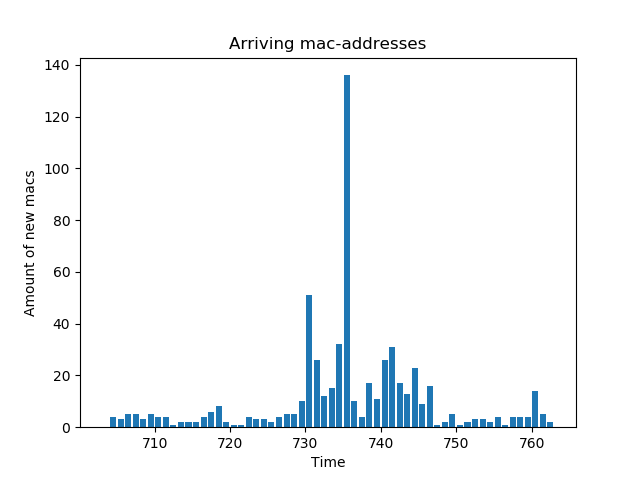
\includegraphics[width=\linewidth]{fridaymorning7-8v2.png}
     \caption{K-Means with wrong datapoints}
	\label{fig:basicbargraph1}
  \end{subfigure}
  \begin{subfigure}[b]{0.3\linewidth}
    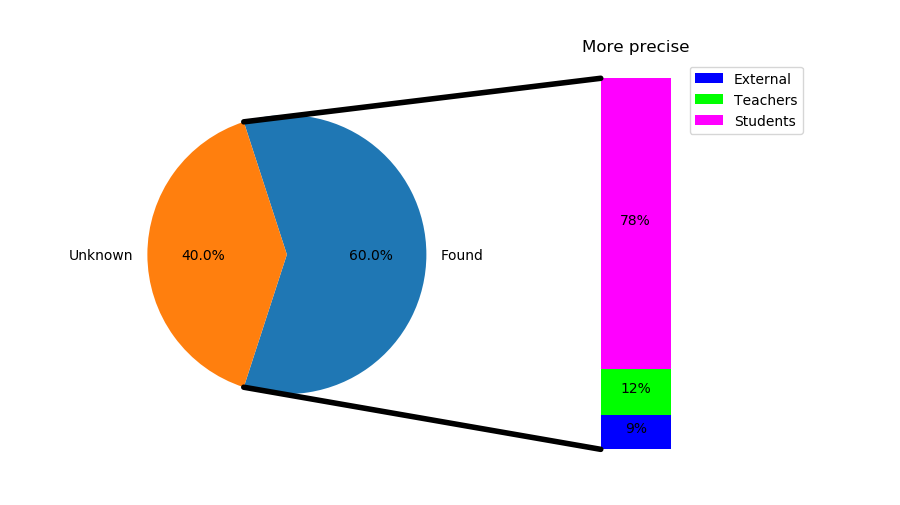
\includegraphics[width=\linewidth]{piecharwith_usernames.png}
    \caption{DBSCAN with wrong datapoints}
 \label{fig:piechar1}
  \end{subfigure}
  \begin{subfigure}[b]{0.3\linewidth}
    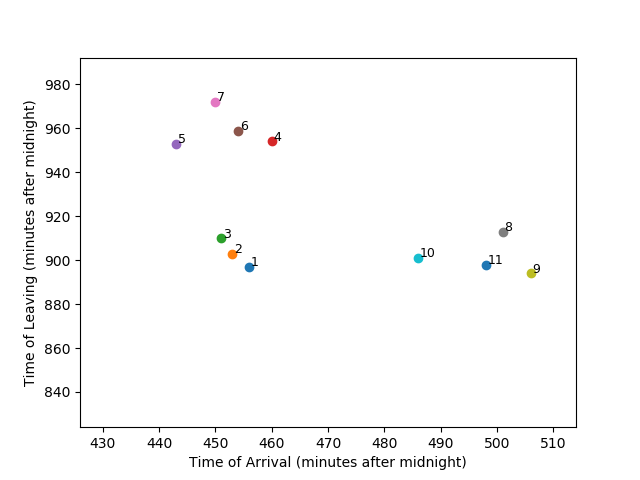
\includegraphics[width=\linewidth]{numbertestset.png}
    \caption{Mean-Shift with wrong points}
\label{fig:numbered1}
  \end{subfigure}
  \begin{subfigure}[b]{0.2\linewidth}
    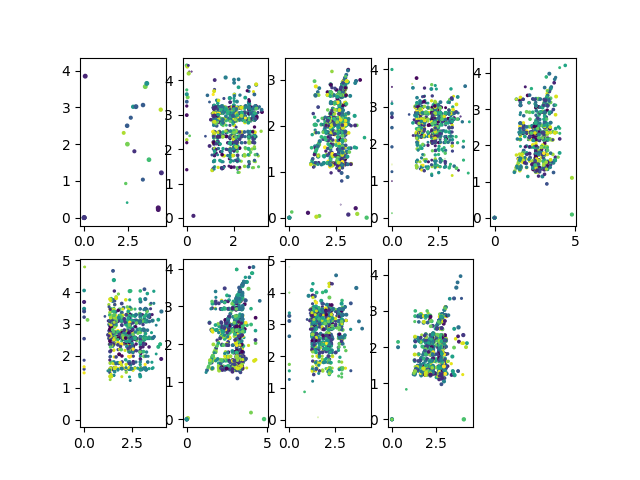
\includegraphics[width=\linewidth]{multiple_dimension_6.png}
  \caption{Numbering a basic scattered graph}
  \label{fig:scattergraph1}
  \end{subfigure}
 \begin{subfigure}[b]{0.2\linewidth}
  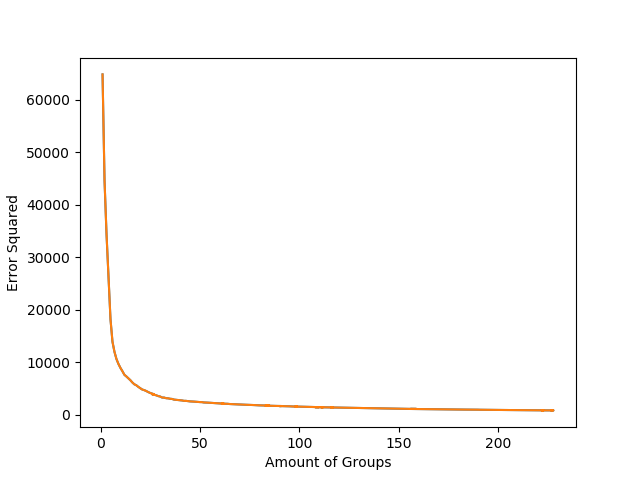
\includegraphics[width=\linewidth]{groupstoerror.png}
  \caption{Relation between amount of group and error}
  \label{fig:line1}
	\end{subfigure}
 \begin{subfigure}[b]{0.2\linewidth}
  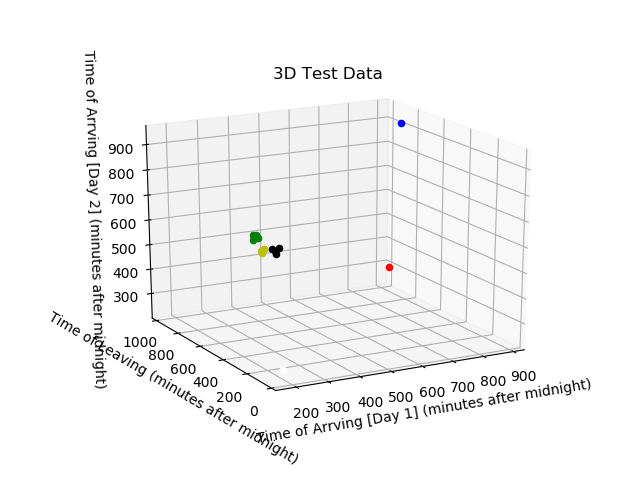
\includegraphics[width=\linewidth]{3Dploting.png}
  \caption{3D ploting}
  \label{fig:3D1}
	\end{subfigure}
  \caption{Same data with different algorithms}
  \label{fig:PoCGraphs}
\end{figure}

Figure \ref{fig:basicbargraph1} shows a simple graph which counts the new mac-addresses per minute. Bar-Graphs help display a lot of different things, not only arrival times. I can figure out how many people stay late, walk by often or go out eat.


The pie char \ref{fig:piechar1} is useful for showing how much of a specific group I can find. In this case, it is how many usernames I could find ou,t and the bar graph helps to make it more exact and more explicit. Later I may add the category PWD or PEAP protocol.


Figure \ref{fig:numbered1} is the first one I did not use my accurate data. But this is more for explaining then actually plotting the real information. I may use it for the real data later, but then I most likely have to go to something like figure \ref{fig:scattergraph1}.


I am not a huge fan of figure \ref{fig:scattergraph1} because it is not very well laid out, but it is still the most transparent way to display more the three dimensions which I am going to use. I doubt it that  figure  \ref{fig:scattergraph1} will make it in the final version. But for 3D the graph \ref{fig:3D1} works fine.


Graph \ref{fig:line1} again an elementary graph, but depending on the algorithm, it can be very useful to display different relations.

I may add some more like the variance box, but I have no data to make a good test. I first need some results.




\section{PoC Algorithms}
\begin{figure}[H]
  \centering
  \begin{subfigure}[b]{0.2\linewidth}
    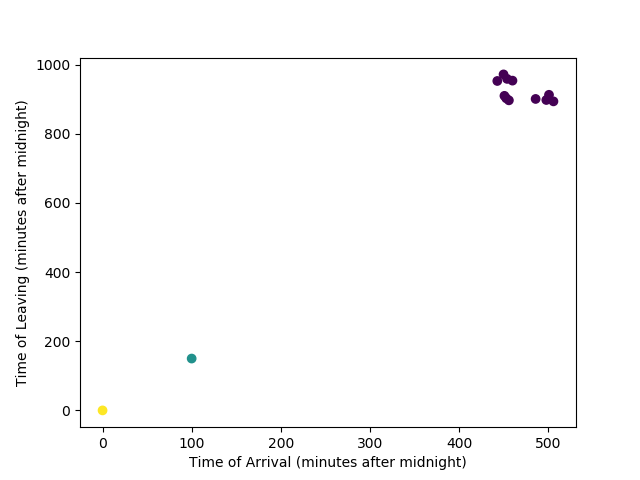
\includegraphics[width=\linewidth]{POC_simple_data_labels_two_wrong_point.png}
     \caption{K-Means with wrong datapoints}
	\label{fig:kmean1}
  \end{subfigure}
  \begin{subfigure}[b]{0.2\linewidth}
    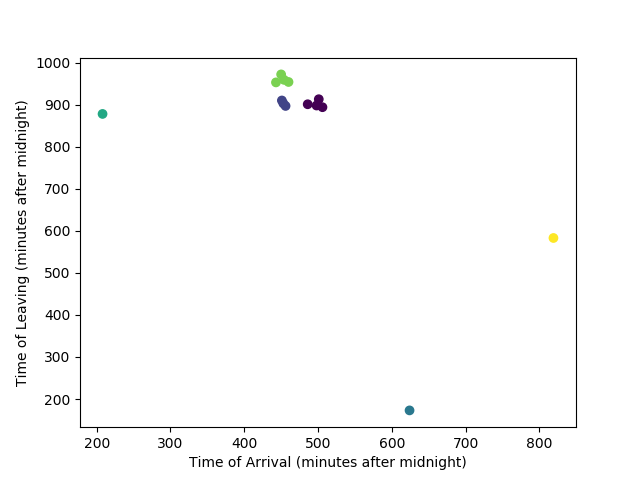
\includegraphics[width=\linewidth]{POC_simple_data_labels_two_wrong_point_dbscan.png}
    \caption{DBSCAN with wrong datapoints}
	\label{fig:dbscan1}
  \end{subfigure}
  \begin{subfigure}[b]{0.2\linewidth}
    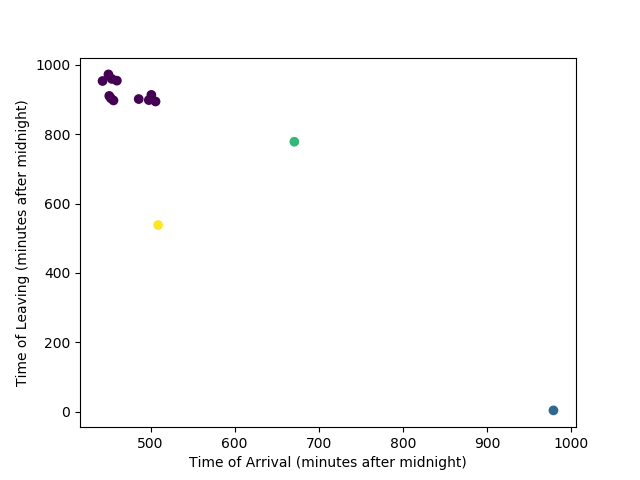
\includegraphics[width=\linewidth]{POC_simple_data_labels_two_wrong_point_mean-shift.png}
    \caption{Mean-Shift with wrong points}
	\label{fig:meanshift1}
  \end{subfigure}
  \caption{Same data with different algorithms}
  \label{fig:pocalgor3}
\end{figure}

I tried different algorithms. I first had high hopes in K-Means, because this would find the groups automatically for me without me giving them the centroids. But because K-Means uses every data-point in the set, I cannot get the right amounts of groups without merging or ripping a group apart (see figure \ref{fig:kmean1}). At the beginning, I had hopes that I could filter the data enough that the noise would fall out. This filtering was not possible without risking to loose relevant data. For comprehensive data, K-Means gets the right groups very nicely, but we don't live in a perfect world. Mean-Shift (Figure \ref{fig:meanshift1}) is very similar to K-Means and therefore also not usable for my data-set without cleaning it up too much. 

I was more lucky with DBSCAN (shown in figure \ref{fig:dbscan1}). For DBSCAN, I cannot give the amount of groups, but I can say how far away the groups are allowed to stretch. In this case, it can find more dens places in the data-cloud. Figure \ref{fig:scattergraph1} shows well that there are denser parts and parts with nearly no data. Therefore I believe this algorithm would work with the full data-set. 



Because I did not just want unsupervised algorithms which work without any given solution set, I tried KNN (K-Nearest-Neighbor). This algorithm calculates the distance between the centroids you provide and groups them to minimize the error distance.

The main difference, as I said, is that I have to provide the central points. This is not hard. I just used a little logic and the time-table and got the time-table.
Then I have to calculate the distance of every point from every class. In my test data-set, I placed a centre point at about point two in figure \ref{fig:numbered1}. The classmates of two had a distance of about 15-100 but everyone else at least 1200. This should work very well. 

Another algorithm I am working on is the decision tree. There I check if I can separate the classes by an only logical basis. This should work for most classes but can be more work then win.


Sorry that the graphics are so small. I tried to bring it all to two pages and with big graphics, this is not possible. (The pictures are in the "Bericht" folder on git.edu-zg.ch) The code-fragments are available on git. The important ones are in Code/advanced algorithm/ and in Code/graphics.

\end{document}

